\documentclass[runningheads]{llncs}

% ---------------------------------------------------------------
% Include basic ECCV package
\usepackage[review,year=2026,ID=10551]{eccv}

% ---------------------------------------------------------------
% Other packages (keep lightweight for ECCV/LLNCS)
\usepackage{eccvabbrv}
\usepackage{graphicx}
\usepackage{booktabs}
\usepackage[accsupp]{axessibility}
\usepackage{multirow}
\usepackage{cite}
\usepackage{color}
\usepackage{amsmath,amssymb}
\usepackage{algorithm}
\usepackage{algorithmic}
\usepackage{hyperref}
\usepackage{orcidlink}
\usepackage{float}
\usepackage{array}
\usepackage{tabularx}
\graphicspath{{./}{PIC/}{fig/}}
\newcommand{\best}[1]{\textcolor{red}{#1}}
\newcommand{\second}[1]{\textcolor{blue}{#1}}

\begin{document}

\title{Supplementary Material: Multi-Condition Underwater Image Enhancement Based on Rectified Flow}
\titlerunning{Supplementary Material}

\author{Liangfan Shi \and Huimin Lu}
\authorrunning{L.~Shi and H.~Lu}

\institute{Southeast University, Jiangsu, China}

\maketitle

\section{Network Architecture Details}
\label{sec:supp_arch}

This section provides a layer-wise description of the proposed RF-MCUIE velocity network $v_{\theta}$ and how multi-condition information is injected to adapt the enhancement dynamics to diverse underwater water types. The official ECCV 2026 code repository is \url{https://github.com/zyc4718/Rectifying-the-Depths}.

\subsection{Multi-condition representation}
\label{sec:supp_cond_rep}

Given a raw underwater input $I_{\mathrm{raw}}\in\mathbb{R}^{H\times W\times 3}$, our preprocessing stage estimates a background light map $B\in\mathbb{R}^{H\times W\times 3}$, a transmission map $T\in\mathbb{R}^{H\times W\times 3}$, and an adaptive reliability mask $\mathcal{M}\in[0,1]^{H\times W}$ as described in Sec.~3 of the main paper. We construct a spatial condition tensor
\begin{equation}
C = \mathrm{Concat}\Bigl(\mathcal{M}\odot I_{\mathrm{raw}},\ \mathcal{M}\odot B,\ \mathcal{M}\odot T\Bigr)\in\mathbb{R}^{H\times W\times 9},
\label{eq:supp_cond_tensor}
\end{equation}
This tensor explicitly preserves the observed degraded appearance together with physics-inspired priors. It is particularly useful in multi-condition settings because different water types induce different attenuation and backscatter statistics, and those variations are reflected in the estimated background light and transmission patterns.

In addition to $C$, we derive a compact global water-type embedding $e_c\in\mathbb{R}^{d}$ to modulate the velocity field at all resolutions:
\begin{equation}
e_c = \mathrm{MLP}\!\left(\mathrm{GAP}\!\left(\phi(C)\right)\right),
\qquad \phi(\cdot):\mathbb{R}^{H\times W\times 9}\rightarrow\mathbb{R}^{H\times W\times d_\phi},
\label{eq:supp_global_cond}
\end{equation}
where $\phi(\cdot)$ is a shallow condition encoder defined in Sec.~\ref{sec:supp_cond_enc}, and $\mathrm{GAP}$ is global average pooling. This embedding summarizes the dominant veiling color, attenuation imbalance, and contrast loss pattern of the input scene.

\subsection{Condition encoder and multi-scale priors}
\label{sec:supp_cond_enc}

We extract multi-scale condition features $\{F^c_s\}_{s=0}^{S}$ that align with the U-Net resolutions. Starting from $C$, the encoder uses strided convolutions to progressively downsample:
\begin{equation}
F^c_{0}=\psi_0(C),\qquad
F^c_{s+1}=\psi_{s+1}\!\left(\mathrm{Down}(F^c_s)\right),
\label{eq:supp_cond_pyramid}
\end{equation}
where each $\psi_s$ is a residual Conv--Norm--SiLU block and $\mathrm{Down}$ is a $3\times 3$ stride-2 convolution. We use $S=3$ levels in practice, matching the 4-stage U-Net, and set channels $\{64,128,256,256\}$ for $\{F^c_0,\dots,F^c_3\}$.

These features serve two purposes. They provide keys and values for cross-attention so that spatial priors can be injected at matched resolutions, and they also provide pooled statistics for constructing $e_c$ in \eqref{eq:supp_global_cond}.

\subsection{Velocity U-Net backbone}
\label{sec:supp_unet}

We parameterize the rectified flow velocity field as a conditional U-Net:
\begin{equation}
v_\theta:\ \left(X_t,\ C,\ t\right)\mapsto \widehat{u}_t\in\mathbb{R}^{H\times W\times 3},
\qquad t\in[0,1],
\end{equation}
where $X_t\in\mathbb{R}^{H\times W\times 3}$ is the current state along the ODE trajectory. The network input is the channel-wise concatenation $[X_t;C]\in\mathbb{R}^{H\times W\times 12}$.

We use a 4-stage U-Net with channel multipliers $\{1,2,4,4\}$ and base width $64$.
Each stage contains two residual blocks, followed by a stride-2 downsample (encoder) or a nearest-neighbor upsample + $3\times 3$ convolution (decoder).
Skip connections concatenate encoder features to decoder features at matching resolutions.

Given an input feature $h\in\mathbb{R}^{H_s\times W_s\times C_s}$, each residual block computes
\begin{equation}
\mathrm{ResBlock}(h;\,e_t,e_c) = h + \mathrm{Conv}_{3\times 3}\!\Bigl(\sigma\bigl(\mathrm{ModGN}(h;\,e_t,e_c)\bigr)\Bigr),
\label{eq:supp_resblock}
\end{equation}
where $\sigma$ is SiLU and $\mathrm{ModGN}$ is a modulation of GroupNorm by time/condition embeddings (Sec.~\ref{sec:supp_inject}). The output is projected to the target channel width if needed via $1\times 1$ convolution.

To model global color cast and long-range haze, we insert attention blocks at the $1/8$ and $1/16$ resolutions after the second and third downsampling stages. At each chosen stage, we apply a self-attention block to the main features and a cross-attention block from main features to the aligned condition features $F^c_s$.

\subsection{Multi-condition injection: time embedding, FiLM, and cross-attention}
\label{sec:supp_inject}

We embed continuous time using sinusoidal features and an MLP:
\begin{equation}
\gamma(t)=\bigl[\sin(\omega_1 t),\cos(\omega_1 t),\dots,\sin(\omega_L t),\cos(\omega_L t)\bigr],
\qquad
e_t = \mathrm{MLP}_t\!\left(\gamma(t)\right)\in\mathbb{R}^{d}.
\label{eq:supp_time_emb}
\end{equation}
We set $L=64$ and $d=256$.

Let $\mathrm{GN}(\cdot)$ denote GroupNorm. We compute scale and shift from the joint embedding $(e_t,e_c)$:
\begin{equation}
\left[s(h),\,b(h)\right] = W_2\,\sigma\!\left(W_1\,[e_t;e_c]\right),
\qquad s(h),b(h)\in\mathbb{R}^{C_s},
\end{equation}
and modulate features channel-wise:
\begin{equation}
\mathrm{ModGN}(h;\,e_t,e_c) = \bigl(1+s(h)\bigr)\odot \mathrm{GN}(h) + b(h).
\label{eq:supp_modgn}
\end{equation}
This modulation makes the velocity field depend directly on the ODE time and on the global water-type signature, allowing the network to adapt its enhancement rate across different degradation regimes.

To inject spatial priors, we attend to condition features $F^c_s$ at the same scale:
\begin{align}
Q &= W_q\,\mathrm{vec}(h),\quad K=W_k\,\mathrm{vec}(F^c_s),\quad V=W_v\,\mathrm{vec}(F^c_s),\\
\mathrm{Attn}(h,F^c_s) &= \mathrm{reshape}\!\left(\mathrm{softmax}\!\left(\frac{QK^\top}{\sqrt{d_a}}\right)V\right),
\end{align}
where $\mathrm{vec}(\cdot)$ flattens spatial dimensions to length $H_sW_s$ and $d_a$ is the attention head width. We apply WTAA in both encoder and decoder attention stages:
\begin{equation}
h \leftarrow h + \mathrm{Attn}(h,F^c_s),
\label{eq:supp_cross_attn_res}
\end{equation}
which empirically improves the stability of multi-condition restoration by aligning the velocity update with physically plausible priors.

\begin{table*}[t]
\centering
\small
\renewcommand{\arraystretch}{1.18}
\setlength{\tabcolsep}{4pt}
\caption{Layer specification of the conditional velocity U-Net. ``FiLM'' denotes ModGN modulation by $(e_t,e_c)$, and ``WTAA'' denotes cross-attention to condition features.}
\label{tab:supp_arch_table}
\begin{tabularx}{\textwidth}{@{}>{\raggedright\arraybackslash}m{0.12\textwidth}>{\centering\arraybackslash}m{0.13\textwidth}>{\centering\arraybackslash}m{0.10\textwidth}>{\raggedright\arraybackslash}m{0.18\textwidth}>{\raggedright\arraybackslash}X>{\raggedright\arraybackslash}m{0.16\textwidth}@{}}
\toprule
Stage & Resolution & Channels & Blocks & Conditioning & Attention \\ \midrule
0 & $H\times W$ & 64  & 2 ResBlocks, then downsample & FiLM in all blocks & None \\
1 & $H/2\times W/2$ & 128 & 2 ResBlocks, then downsample & FiLM in all blocks & None \\
2 & $H/4\times W/4$ & 256 & 2 ResBlocks, then downsample & FiLM and WTAA & Self-attention and cross-attention \\
3 & $H/8\times W/8$ & 256 & 2 ResBlocks & FiLM and WTAA & Self-attention and cross-attention \\
Bottleneck & $H/8\times W/8$ & 256 & 2 ResBlocks & FiLM & Self-attention \\
Decoder & Symmetric & -- & Upsample, skip fusion, ResBlocks & FiLM throughout, WTAA at Stages 2--3 & Self-attention and cross-attention at Stages 2--3 \\
\bottomrule
\end{tabularx}
\end{table*}

\section{Conditional Rectified Flow: Training and Sampling Pseudocode}
\label{sec:supp_algo}

Rectified flow learns a nearly straight transport from a simple source distribution $\pi_0$, represented as Gaussian noise, to the conditional target distribution $\pi_1(\cdot\,|\,C)$.
We provide pseudocode for both training (velocity regression) and sampling (ODE integration).

\subsection{Training objective recap}
We sample $X_0\sim\mathcal{N}(0,\mathbf{I})$ and define the linear interpolation between source and target enhanced image $J$:
\begin{equation}
X_t = (1-t)X_0 + tJ,\qquad t\sim\mathcal{U}[0,1],
\label{eq:supp_interp}
\end{equation}
which yields a target velocity $u_t = \frac{dX_t}{dt} = J - X_0$.
The network minimizes a masked velocity regression loss described in the main paper:
\begin{equation}
\mathcal{L}_{\mathrm{vel}} = \bigl\|\mathcal{M}\odot\bigl(v_\theta(X_t,C,t) - (J-X_0)\bigr)\bigr\|_2^2.
\end{equation}

\subsection{Algorithm}
Algorithm~\ref{alg:supp_train} summarizes the training pipeline, and Algorithm~\ref{alg:supp_sample} gives the corresponding sampling procedure.

\begin{algorithm}[H]
\caption{Conditional Rectified Flow Training (RF-MCUIE)}
\label{alg:supp_train}
\begin{algorithmic}[1]
\REQUIRE Paired training set $\{(I_{\mathrm{raw}},J)\}$, iterations $K$, batch size $B$, base step number $N_{\mathrm{train}}$.
\STATE Initialize parameters $\theta$ of $v_\theta$ and preprocessing modules.
\FOR{$k=1$ to $K$}
    \STATE Sample a minibatch $\{(I_{\mathrm{raw}}^{(i)},J^{(i)})\}_{i=1}^{B}$.
    \STATE Estimate physical priors and mask: $(B^{(i)},T^{(i)},\mathcal{M}^{(i)})\leftarrow \mathrm{Preprocess}(I_{\mathrm{raw}}^{(i)},J^{(i)})$.
    \STATE Construct conditions $C^{(i)}$ using \eqref{eq:supp_cond_tensor}.
    \STATE Sample $t^{(i)}\sim \mathcal{U}[0,1]$ and noise $X_0^{(i)}\sim \mathcal{N}(0,\mathbf{I})$.
    \STATE Interpolate $X_t^{(i)} \leftarrow (1-t^{(i)})X_0^{(i)} + t^{(i)}J^{(i)}$.
    \STATE Target velocity $u_t^{(i)}\leftarrow J^{(i)}-X_0^{(i)}$.
    \STATE Predict $\widehat{u}_t^{(i)} \leftarrow v_\theta(X_t^{(i)}, C^{(i)}, t^{(i)})$.
    \STATE Compute masked regression loss $\mathcal{L}_{\mathrm{vel}}$ and update $\theta$ by back-propagation.
    \IF{two-stage fine-tuning enabled}
        \STATE Optionally integrate $X_0\rightarrow X_1$ with $N_{\mathrm{train}}$ Euler steps and apply image-domain losses on $X_1$.
    \ENDIF
\ENDFOR
\end{algorithmic}
\end{algorithm}

\begin{algorithm}[H]
\caption{Conditional Rectified Flow Sampling (Euler Integration)}
\label{alg:supp_sample}
\begin{algorithmic}[1]
\REQUIRE Raw input $I_{\mathrm{raw}}$, step number $N$, trained parameters $\theta$.
\STATE Obtain priors and condition tensor $C\leftarrow \mathrm{Preprocess}(I_{\mathrm{raw}})$.
\STATE Initialize $X_0\sim\mathcal{N}(0,\mathbf{I})$.
\STATE Set $\Delta t \leftarrow 1/N$.
\FOR{$k=0$ to $N-1$}
    \STATE $t_k \leftarrow k\Delta t$.
    \STATE $X_{k+1} \leftarrow X_k + \Delta t\cdot v_\theta(X_k,C,t_k)$.
\ENDFOR
\STATE Output enhanced image $\widehat{J}\leftarrow X_N$.
\end{algorithmic}
\end{algorithm}

\section{Implementation Details}
\label{sec:supp_impl}

We follow the main paper for dataset splits and paired/unpaired usage. During training, images are randomly cropped to $256\times 256$ and augmented by random horizontal/vertical flips and $90^\circ$ rotations.

Unless specified otherwise, we use Adam with $(\beta_1,\beta_2)=(0.9,0.999)$, initial learning rate $1\times 10^{-4}$, and batch size 8.
We employ a linear warm-up for the first 10k iterations followed by cosine decay to $1\times 10^{-6}$.
Weight decay is set to $1\times 10^{-4}$ and gradient clipping is applied at 1.0.

The velocity regression loss is always enabled. In the second-stage fine-tuning, we additionally use a composite image-domain loss composed of $\ell_1$, perceptual, and color-consistency terms with weights $\lambda_{\mathrm{rec}}=1.0$, $\lambda_{\mathrm{perc}}=0.1$, and $\lambda_{\mathrm{color}}=0.05$.

We set $N_{\mathrm{train}}=1$ for stable and efficient training and use $N\in\{1,3,5,10\}$ for the inference-time trade-off analysis reported in Sec.~\ref{sec:supp_speed_quality}.

All models are trained on a single NVIDIA RTX A6000 GPU. Unless otherwise noted, inference is benchmarked on full-resolution $512\times 512$ images with batch size 1.

\section{Neural ODE Trajectory Visualization}
\label{sec:supp_ode_vis}

Rectified flow defines a deterministic neural ODE $\frac{dX_t}{dt}=v_\theta(X_t,C,t)$ that transports samples from $\pi_0$ to $\pi_1(\cdot|C)$.
Figure~\ref{fig:supp_ode_schematic} gives a concept-level view of the conditional transport process, while Figure~\ref{fig:supp_ode_real} shows how a real underwater sample evolves from the degraded input toward the restored output. The first figure is used to visualize the condition-dependent flow behavior in a compact synthetic setting. The second figure is built from the actual input-output pair in the repository and presents a deterministic progression of intermediate image states together with a low-dimensional trajectory measured by image statistics.

\begin{figure*}[t]
\centering
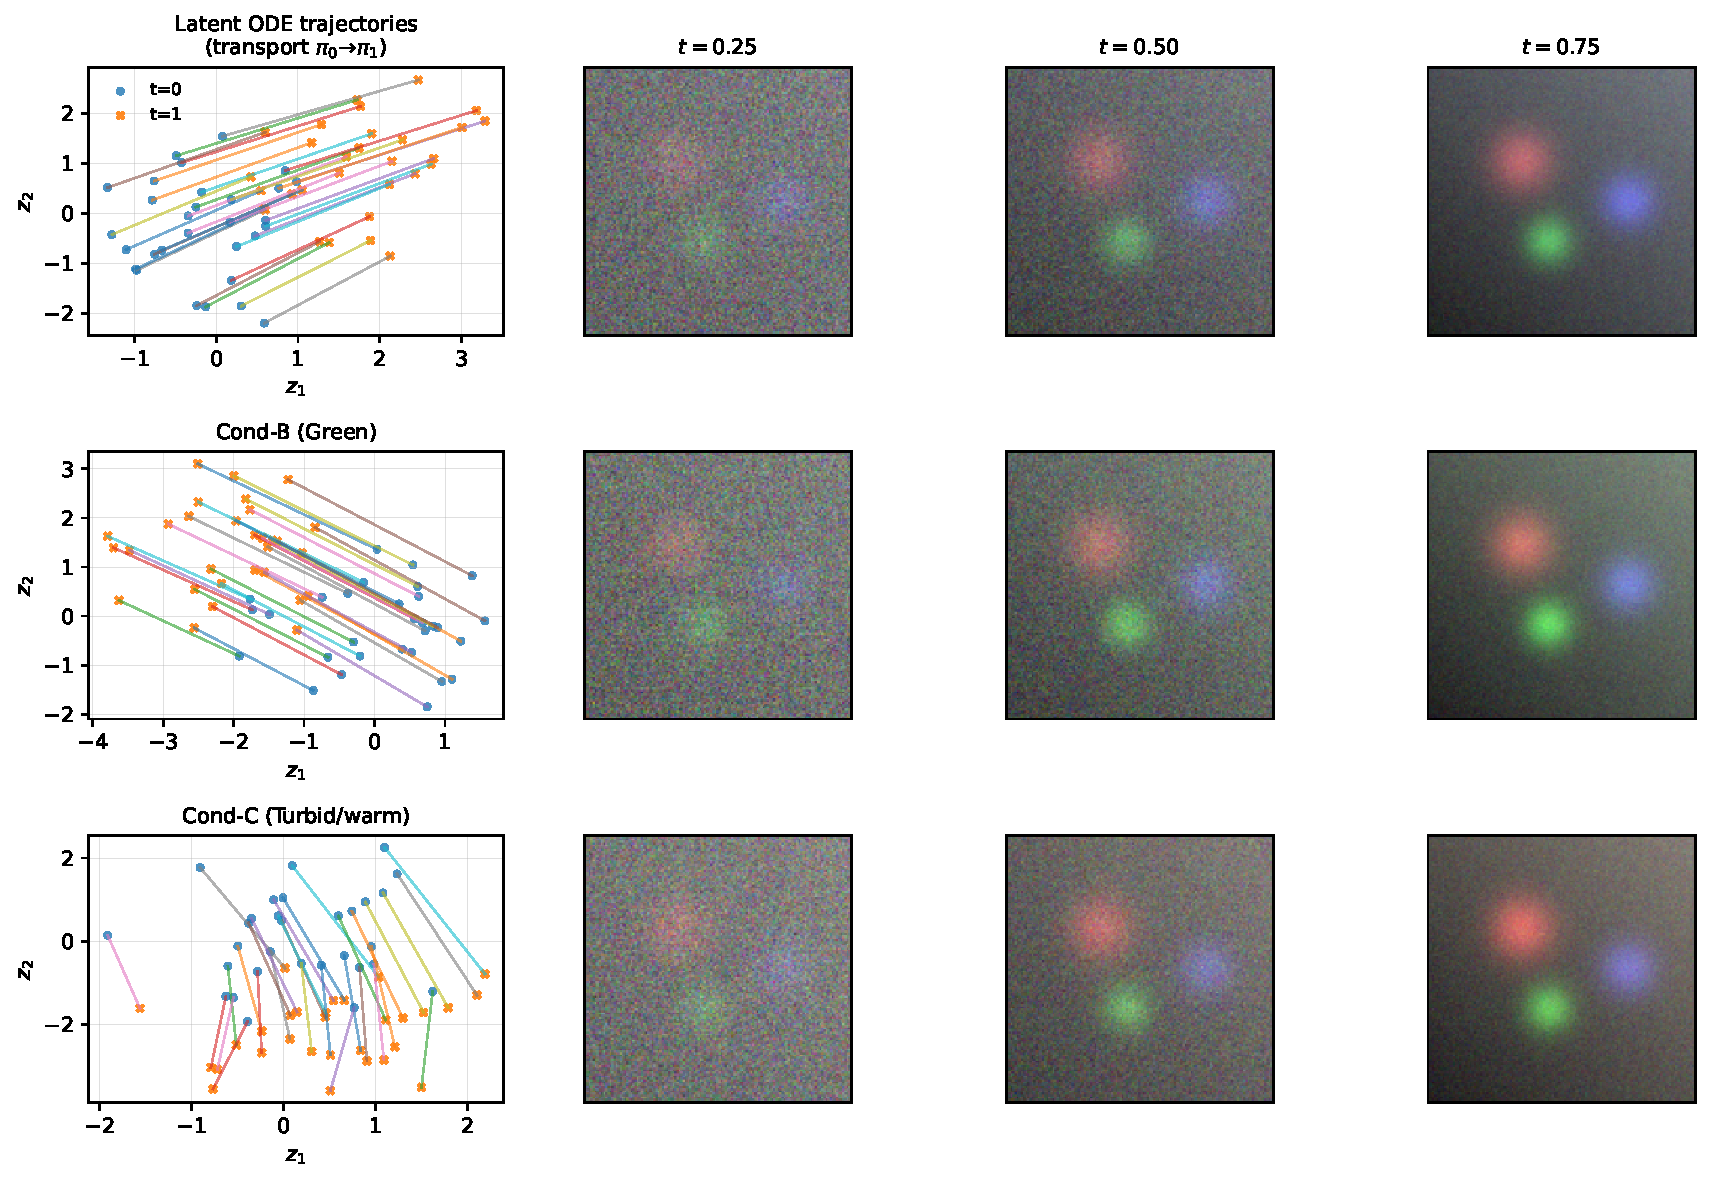
\includegraphics[width=\linewidth]{rf_ode_trajectories.pdf}
\caption{Schematic visualization of rectified-flow ODE transport under different condition vectors. The left column shows toy latent trajectories from $\pi_0$ to $\pi_1$, and the right columns visualize representative intermediate states along the transport path.}
\label{fig:supp_ode_schematic}
\end{figure*}

\begin{figure*}[t]
\centering
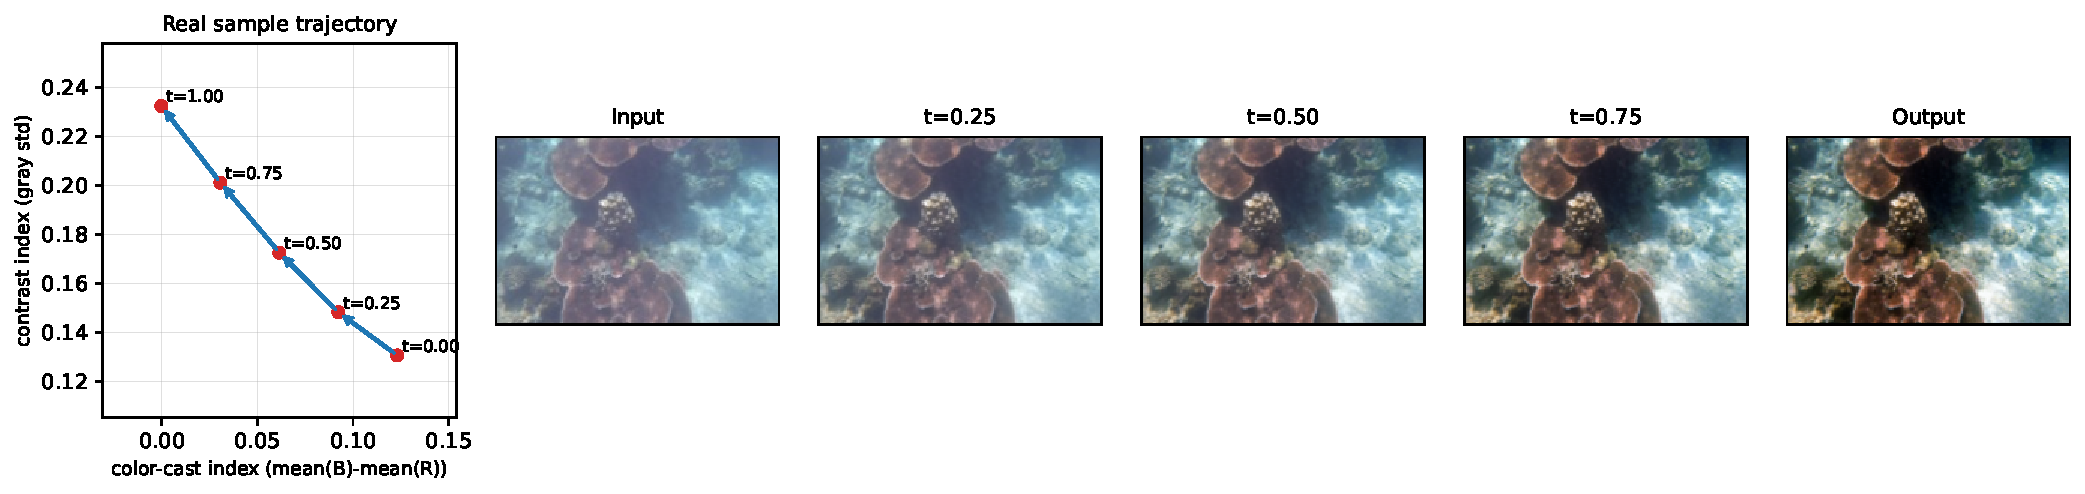
\includegraphics[width=\linewidth]{rf_ode_real_case.pdf}
\caption{Real-sample trajectory and intermediate image states built from the repository input-output pair. The left panel plots the progression in a two-dimensional image-statistic space using the color-cast index $\mathrm{mean}(B)-\mathrm{mean}(R)$ and the grayscale contrast standard deviation. The right panels show the corresponding image states at $t=0.00, 0.25, 0.50, 0.75$, and $1.00$.}
\label{fig:supp_ode_real}
\end{figure*}

\section{Additional Qualitative Results}
\label{sec:supp_qual}

Figure~\ref{fig:supp_qual_grid} provides a broader qualitative comparison across six additional underwater scenes and complements the representative examples in the main paper. The rows cover green-dominant color casts, bluish scattering, low-contrast seabed scenes, and cases in which local detail recovery is particularly difficult. Across these varied degradations, the proposed RF-MCUIE produces more balanced visibility enhancement and color correction than competing baselines.

\begin{figure*}[t]
\centering
\includegraphics[width=\linewidth]{fig_supp_overall_comparison.png}
\caption{Additional qualitative comparison under diverse underwater degradations. The columns are Raw, ZAP, ICSP, UIE-WD, DM-water, LANet, UIEC2Net, and Ours.}
\label{fig:supp_qual_grid}
\end{figure*}

Traditional methods such as ZAP and ICSP often leave under-corrected colors or insufficient contrast restoration when scattering becomes severe. Learning-based baselines such as UIE-WD and DM-water improve visibility in several scenes, but residual color drift and locally unstable enhancement remain visible in challenging regions. LANet and UIEC2Net recover stronger textures in some examples, yet their global color tone is less stable across all rows. In contrast, RF-MCUIE better suppresses residual casts, restores scene visibility, and preserves the underlying structures with fewer obvious artifacts, which is consistent with the quantitative advantages reported in the main paper.

\section{Additional Quantitative Results}
\label{sec:supp_quant}

\subsection{Extended benchmark summary across datasets}
Table~\ref{tab:supp_quant_all} summarizes the main quantitative metrics across multiple datasets in a unified format.

\begin{table*}[t]
\centering
\small
\caption{Extended quantitative summary across datasets. Values are taken from the main paper tables for consistent comparison. ``--'' indicates metrics that are not defined for the corresponding dataset because paired references are unavailable.}
\label{tab:supp_quant_all}
\begin{tabular}{@{}l l c c c c@{}}
\toprule
Dataset & Method & PSNR $\uparrow$ & SSIM $\uparrow$ & UCIQE $\uparrow$ & UIQM $\uparrow$ \\ \midrule
\multirow{4}{*}{LSUI} 
    & UIEC$^2$-Net & 22.96 & 0.86 & \best{0.60} & \second{3.06} \\
    & U-shape      & 24.83 & 0.87 & 0.56 & \best{3.08} \\
    & DM-water     & \best{25.12} & \second{0.88} & 0.57 & 2.90 \\
    & \textbf{Ours}           & \textbf{\second{24.91}} & \textbf{\best{0.90}} & \textbf{\second{0.59}} & \textbf{2.98} \\ \midrule
\multirow{4}{*}{UIEB} 
    & UIEC$^2$-Net & \best{23.82} & \best{0.87} & \best{0.61} & \second{3.05} \\
    & U-shape      & 22.17 & \second{0.82} & 0.57 & \best{3.10} \\
    & DM-water     & 21.64 & \second{0.82} & 0.57 & 2.86 \\
    & \textbf{Ours}           & \textbf{\second{23.18}} & \textbf{\best{0.87}} & \textbf{\second{0.58}} & \textbf{2.91} \\ \midrule
\multirow{4}{*}{U45} 
    & UIEC$^2$-Net & -- & -- & \second{0.61} & \best{3.40} \\
    & LANet        & -- & -- & \best{0.63} & 3.29 \\
    & DM-water     & -- & -- & 0.60 & 3.26 \\
    & \textbf{Ours}           & -- & -- & \textbf{\second{0.61}} & \textbf{\second{3.32}} \\ \bottomrule
\end{tabular}
\end{table*}

\subsection{Speed--quality trade-off on full-resolution inference}
\label{sec:supp_speed_quality}

Table~\ref{tab:supp_speed_quality} reports the trade-off between inference steps $N$, runtime, and quality metrics on our $512\times 512$ benchmark. In practice, $N=3$ offers an excellent speed--quality balance.

\begin{table*}[t]
\centering
\small
\caption{Speed--quality trade-off of RF-MCUIE at $512\times 512$ resolution with batch size 1 on an NVIDIA RTX A6000.}
\label{tab:supp_speed_quality}
\begin{tabular}{@{}c c c c c c c c@{}}
\toprule
Steps $N$ & Time (ms/img) $\downarrow$ & PSNR $\uparrow$ & SSIM $\uparrow$ & UCIQE $\uparrow$ & UIQM $\uparrow$ & LPIPS $\downarrow$ & FID $\downarrow$ \\
\midrule
1  & \best{98.85}  & 23.17 & 0.858 & 0.583 & \best{3.153} & 0.0596 & 29.99 \\
3  & \second{292.38} & \best{23.71} & \second{0.870} & \second{0.587} & \second{3.046} & \second{0.0494} & \second{24.86} \\
5  & 486.56 & \second{23.68} & \best{0.872} & \second{0.587} & 3.038 & \best{0.0491} & 24.90 \\
10 & 976.50 & 23.67 & 0.869 & \best{0.589} & 3.022 & 0.0509 & \best{24.85} \\
\bottomrule
\end{tabular}
\end{table*}

\section{Comprehensive Ablation Studies}
\label{sec:supp_ablation}

We further analyze the effect of multi-condition injection and training strategy.

\subsection{Efficacy of multi-condition injection}
Table~\ref{tab:supp_ablation_modules}, reproduced from the main paper for convenience, shows that injecting multi-condition priors significantly improves perceptual quality and fidelity.
Comparing Model~I and Model~II verifies that conditioning on $(I_{\mathrm{raw}},B,T)$ is essential for handling diverse water types.

\begin{table}[t]
\centering
\small
\caption{Ablation of key components including multi-condition injection, the two-stage loss, and ADMK.}
\label{tab:supp_ablation_modules}
\begin{tabular}{@{}l c c c c c c c@{}}
\toprule
Model & Cond. & Two-Stage & ADMK & UCIQE $\uparrow$ & UIQM $\uparrow$ & PSNR $\uparrow$ & SSIM $\uparrow$ \\ \midrule
Model I   & $\times$ & $\times$ & $\times$ & 0.55 & 2.84 & 24.12 & 0.84 \\
Model II  & \checkmark & $\times$ & $\times$ & \second{0.58} & \second{2.92} & 24.37 & 0.86 \\
Model III & \checkmark & \checkmark & $\times$ & 0.57 & 2.90 & \best{25.05} & \best{0.91} \\
\midrule
\textbf{Model IV (Ours)} & \checkmark & \checkmark & \checkmark & \textbf{\best{0.59}} & \textbf{\best{2.98}} & \textbf{\second{24.91}} & \textbf{\second{0.90}} \\
\bottomrule
\end{tabular}
\end{table}

\subsection{Where to inject conditions}
From an architectural viewpoint, multi-condition information can be injected at different depths. Our design combines early concatenation $[X_t;C]$ to preserve pixel-level priors with FiLM modulation and WTAA at deeper layers so that the global dynamics and spatial restoration focus can be adapted jointly.
Empirically, removing either FiLM or WTAA degrades color correction and leads to over/under-enhancement under extreme water types.

\section{Limitations}
\label{sec:supp_limitations}

The proposed framework still depends on the quality of the estimated priors. When background light or transmission estimation fails under strong artificial illumination or severe specular reflections, the resulting conditioning can bias the restoration trajectory and leave residual color shifts. Generalization also becomes harder for rare water compositions and unusual camera responses that are underrepresented during training. In addition, the current model is designed primarily for scattering and attenuation removal, so extremely low-light scenes and heavy motion blur may require extra modules for noise suppression or blur-aware restoration.

Future work will focus on more robust prior estimation under complex lighting, better generalization to unseen water types and camera domains, and tighter integration of enhancement with low-light denoising and motion-blur removal. We also plan to study adaptive step allocation so that the rectified-flow trajectory can preserve the current speed advantage while improving restoration quality in the most difficult scenes.

\end{document}
